\documentclass{amsart}
\usepackage{xcolor,tikz}
\usetikzlibrary[positioning]

\begin{document}

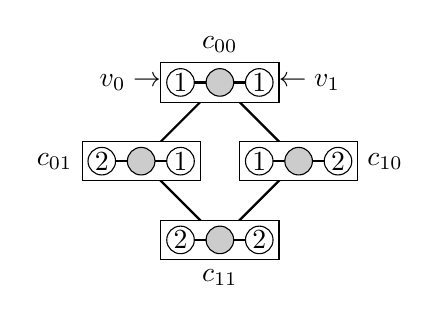
\begin{tikzpicture}[baseline=0cm, scale=0.5]
\draw[style=thick] (5,0)--(3,-2)--(5,-4)--(7,-2)--(5,0);

\draw[fill=white] (3.5,-.5) rectangle (6.5,.5);
\node[anchor=south] at (5,.5) {${c_{00}}$};
\draw[style=thick](4,0)--(6,0);
\draw[radius=.35,fill=white](4,0)circle node{1};
\draw[radius=.35,fill=black!20](5,0)circle;%
\draw[radius=.35,fill=white](6,0)circle node{1};
\node[anchor=east] at (3.75,0) {$v_0\rightarrow$};
\node[anchor=west] at (6.25,0) {$\leftarrow v_1$};

\draw[fill=white] (1.5,-2.5) rectangle (4.5,-1.5);
\node[anchor=east] at (1.5,-2) {${c_{01}}$};
\draw[style=thick](2, -2)--(4,-2);
\draw[radius=.35,fill=white](2,-2)circle node{2};
\draw[radius=.35,fill=black!20](3,-2)circle;
\draw[radius=.35,fill=white](4,-2)circle node{1};

\draw[fill=white] (5.5,-2.5) rectangle (8.5,-1.5);
\node[anchor=west] at (8.5,-2) {$c_{10}$};
\draw[style=thick](8, -2)--(6,-2);
\draw[radius=.35,fill=white](6,-2)circle node{1};
\draw[radius=.35,fill=black!20](7,-2)circle;
\draw[radius=.35,fill=white](8,-2)circle node{2}; 

\draw[fill=white] (3.5,-4.5) rectangle (6.5,-3.5);
\node[anchor=north] at (5,-4.5) {${c_{11}}$};
\draw[style=thick](4,-4)--(6,-4);
\draw[radius=.35,fill=white](4,-4)circle node{2};
\draw[radius=.35,fill=black!20](5,-4)circle;
\draw[radius=.35,fill=white](6,-4)circle node{2}; 
\end{tikzpicture}

\end{document}